\documentclass[]{article}

\usepackage{tabularx}
\usepackage[dutch]{babel}
\usepackage{amsmath}
\usepackage{graphicx}
\usepackage{amsmath}
\usepackage{epstopdf}
\usepackage[parfill]{parskip}

\newcommand{\opgave}[1]{\section*{Opgave #1}}

\begin{document}

\opgave5



Aangezien we hier de gelijktijdige iteratie uitvoeren met I als de start matrix is deze methode hetzelfde als de QR methode zonder shifts. Deze convergeert dus linear net zoals de methode van de machten. De QR methode met rayleigh quotient shift convergeert cubisch. Deze methode is eigenlijk dezelfde methode als de rayleigh iteratie, maar dan in Matrix vorm. Daarom is het ook logisch dat het convergentiegedrag analoog is.
Het nadeel van Rayleigh iteratie is dat je convergeert naar een eigenwaarde die in de buurt ligt van de gekozen startwaarde. Het is niet mogelijk om alle eigenwaarden en eigenvectoren van een matrix te berekenen zonder al een redelijke schatting van iedere eigenwaarde te hebben.

Figuur ~\ref{opgave5} toont de convergentie van de besproken methodes. 

\begin{figure}[h]
\noindent 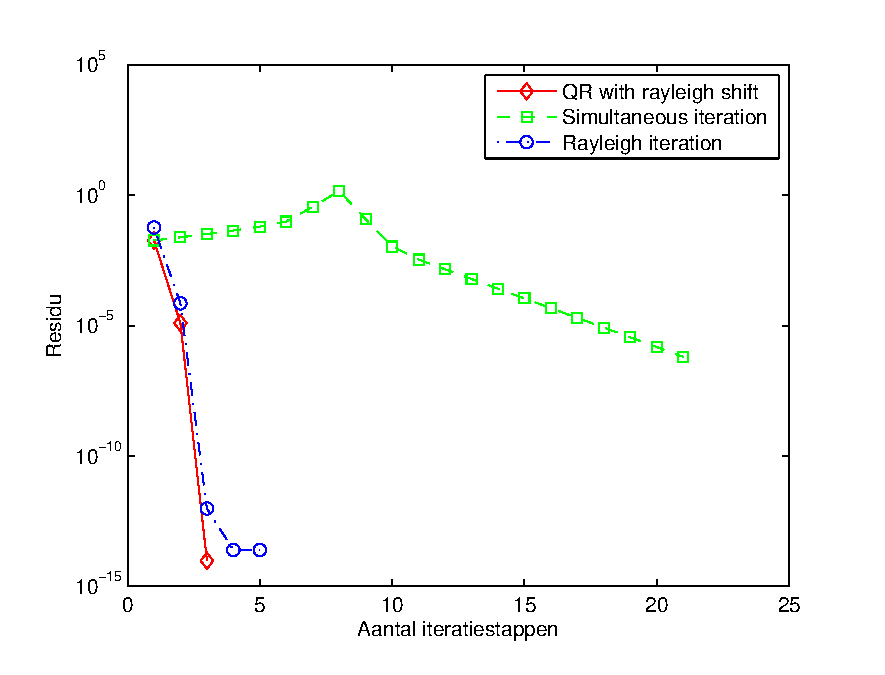
\includegraphics[width=1\linewidth]{opgave5.eps}
\caption{Convergentie van rayleigh iteratie, QR methode met rayleigh shifts en simultane iteratie naar \'{e}\'{e}n eigenwaarde}
\label{opgave5}
\end{figure}
\end{document}